\documentclass[12pt]{report}
\usepackage[utf8]{inputenc}
\usepackage{graphicx}
\usepackage{amsmath}
\usepackage{amsfonts}
\usepackage{cancel}
\usepackage[titletoc]{appendix}
\graphicspath{ {images/} }
\tolerance=1
\emergencystretch=\maxdimen
\hyphenpenalty=10000
\hbadness=10000

\begin{document}

\thispagestyle{empty}
\begin{center}
    \Huge
    \textbf{Field Theoretical Effects of Condensed Matter Systems}\\
    \vspace{1.5cm}
    \textbf{by}\\
    \vspace{0.5cm}
    \textbf{Sombit Roy}
    \vfill
    A thesis presented for the degree of\\
    M.Sc.\\
    \vspace{0.5cm}
    \Large Department of Physics\\
    Birla Institute of Technology and Science, Pilani
    
\end{center}

\chapter*{Acknowledgements}
\addcontentsline{toc}{chapter}{\numberline{}Acknowledgements}
I would like to thank all the faculty in the Physics Department of BITS Pilani. This thesis would not have been possible without the invaluable knowledge they imparted to me. In particular, I am immensely grateful to my supervisor, Prof. Jayendra Nath Bandyopadhyay for his help and advice related to my work. 

\chapter*{Abstract}
\addcontentsline{toc}{chapter}{\numberline{}Abstract}
Historically, field theory has most successfully been applied to the physics of subatomic particles. This branch, Quantum Field Theory, has combined special relativity with quantum mechanics to give extraordinarily accurate results, explaining a vast range of phenomena from the existence of antimatter to the Higgs field. \\ 

\noindent Statistical mechanics and condensed matter physics, on the other hand, have totally different origins. They are related to thermodynamics, the theory of gases, phase transitions, etc. At first glance, it would seem that the two have nothing in common. \\ 

\noindent Things become much more interesting if we see two equations that often arise while studying these `unrelated' subjects. The computation of path integral averages in QFT is done as,

$$\langle A\rangle= \frac{\int \mathcal{D}\phi \,A \,e^{\frac{-S[\phi]}{\hbar}}}{\int \mathcal{D}\phi \,e^{\frac{-S[\phi]}{\hbar}}}$$ 

\noindent while in SM, thermal expection values are of the form,

$$\langle A\rangle= \frac{\sum A \,e^{\frac{-E[\phi]}{k_BT}}}{\sum \,e^{\frac{-E[\phi]}{k_BT}}}$$ \\

\noindent It immediately becomes clear that there is a relation between the two. This is just the tip of the iceberg, there are a multitude of ways in which these two theories are initimately intertwined. In this thesis, I will study the field theoretical effects of condensed matter systems. \\

\noindent The thesis is broadly divided into three parts. The first one covers the fundamentals of QFT. The focus will remain on the $\phi^4$ theory, its manifestation as a field theory using Lagrangian mechanics, its path integral formulation and its perturbative interactions expressed as Feynman diagrams. \\

\noindent The second part covers condensed matter physics, especially the Ising model of a ferromagnet. The above field theory is very similar to the Hamiltonian of the Ising model, and thus analogies can be drawn between QFT and SM. This part also dives into phase transitions and the critical exponents of this model and their derivation using field theory. The concept of scaling is also explored via renormalization group.\\

\noindent Finally, in the third part, I will shift my focus away from the Ising model to study other statistical systems using fields. A vast array of phenomena come under condensed matter physics, but I will keep it limited to the study of Fermi gases and Goldstone bosons.\\

\noindent Note: From here on, throughout the text I have used $\hbar=c=k_B=1$.

\tableofcontents

\part{Methodologies in Field Theory : $\phi^4$ theory}

\chapter{Classical Field Theory}
Fields, in a very basic sense, are entities which are described continuously on a manifold. Their values might be real or imaginary. At a single point on a manifold, they might be represented as a scalar, a vector or a tensor. The manifold itself can be of various forms, like Euclidean or Minkowski. \\

\noindent Thus fields extend themselves naturally to QFT, as spacetime, according to our current understanding, is essentially continuous. The Langrangian formulation of mechanics is easily extrapolated to these continuous fields.

\section{Principle of Least Action}
In field theory, instead of working with the Lagrangian, we work with the Lagrangian density $\mathcal{L}$, defined as $L=\int\mathcal{L}\, dV$. This allows us to express action in the form of spacetime variables. The Lagrangian density is a function of a generalized field, $\eta$, its dreivative, $\partial_\nu\eta$ and the spacetime variables, $x^\nu$. The principle of least action extremizes the action.

$$\delta S=\delta\int L\, dt=\delta\int\mathcal{L}\, dVdt=\delta\int\mathcal{L}\, dx^\nu$$

\noindent For any path, extremum or not, the end points must be fixed, i.e. its variation is zero on the $(d-1)$ dimensional surface bounding the $d$ dimensional integration volume. Therefore, for a path with parameter $\alpha$, we have $\eta(x^\nu;\alpha)=\eta(x^\nu;0)+\alpha\xi(x^\nu)$. $\xi$ vanishes at end points. The action is an extremum for $\eta(x^\nu;0)$, therefore its derivative w.r.t. $\alpha$ also vanishes.

$$\frac{dS}{d\alpha}=\int \left[\frac{\partial\mathcal{L}}{\partial\eta}\frac{\partial\eta}{\partial\alpha}+\frac{\partial\mathcal{L}}{\partial(\partial_\nu\eta)}\frac{\partial(\partial_\nu\eta)}{\partial\alpha}\right]\, d^dx$$

\noindent Integrating by parts,
$$\frac{dS}{d\alpha}=\int \left[\frac{\partial\mathcal{L}}{\partial\eta}-\frac{d}{dx^\nu}\left(\frac{\partial\mathcal{L}}{\partial(\partial_\nu \eta)}\right) \right]\, d^dx + \cancelto{0}{\int\frac{d}{dx^\nu}\left(\frac{\partial\mathcal{L}}{\partial(\partial_\nu \eta)}\frac{\partial\eta}{\partial\alpha}\right)\, d^dx}$$

\noindent The second term vanishes because we transform the $d$ dimensional divergence theorem into an integral over the surface bounding the region of integration, which is zero because the variation of $\eta$ is zero on the surface.

$$\frac{dS}{d\alpha}=0\implies \frac{\partial\mathcal{L}}{\partial\eta}=\frac{d}{dx^\nu}\left(\frac{\partial\mathcal{L}}{\partial(\partial_\nu \eta)}\right)$$

\noindent This is the Euler-Lagrange equation for fields.

\section{Noether's Theorem}
Noether's theorem is quite possibly the single most important theory for fields. It states that for every continuous symmetry there exists a corresponding conservation law. This simple statement has profound implications, as we can derive the basic laws of mechanics simply by observing a symmetry in the system. I will first derive the result, and then see how a symmetry paves the way for conservation laws.\\

\noindent An infinitesimal tranformation is given as $\eta(x^\mu)\rightarrow\eta'(x^{\mu'})=\eta(x^\mu)+\delta\eta(x^\mu)$. If there is no change in coordinates, but only in the functional form of the field variable, then we define $\eta'(x^{\mu})=\eta(x^\mu)+\bar\delta\eta(x^\mu)$. (Note: $\delta\eta(x^\mu) \neq \bar\delta\eta(x^\mu)$)\\

\noindent Action must be invariant under transformation.

$$\int_{\Omega'}d^dx\,\mathcal{L}(\eta',\partial_{\nu'}\eta',x^{\nu'})-\int_{\Omega}d^dx\,\mathcal{L}(\eta,\partial_\nu\eta,x^\nu)=0$$

\noindent $x^{\nu'}$ is a dummy variable but therefore we can change it to $x^\nu$. But still, the domains of integration are different. $\Omega$ and $\Omega'$ differ infinitesimally.

$$\implies\int_{\Omega}d^dx\,\left[(\mathcal{L}(\eta',\partial_\nu\eta',x^\nu)-\mathcal{L}(\eta,\partial_\nu\eta,x^\nu))+\frac{d}{dx^\mu}(\mathcal{L}(\eta,\partial_\nu\eta,x^\nu)\delta x^\mu)\right]=0$$

\noindent Now, we can evaluate the first term as,

\begin{align*}
    \begin{split}
        \mathcal{L}(\eta',\partial_\nu\eta',x^\nu)-\mathcal{L}(\eta,\partial_\nu\eta,x^\nu)&=\frac{\partial\mathcal{L}}{\partial\eta}\bar\delta\eta+\frac{\partial\mathcal{L}}{\partial(\partial_\nu\eta)} \bar\delta(\partial_\nu\eta)\\
        &=\frac{d}{dx^\nu}\left(\frac{\partial\mathcal{L}}{\partial(\partial_\nu\eta)}\right)\bar\delta\eta+\frac{\partial\mathcal{L}}{\partial(\partial_\nu\eta)}\frac{d(\bar\delta\eta)}{dx^\nu}\\
        &=\frac{d}{dx^\nu}\left(\frac{\partial\mathcal{L}}{\partial(\partial_\nu\eta)}\bar\delta\eta\right)
    \end{split}
\end{align*}

\noindent Here, in the second line I have made use of the fact that $\bar\delta$ commutes with $\partial_\nu$ and their order can be interchanged, as it is a change at fixed $x^\nu$, unlike $\delta$. I have also used the Euler Lagrange equation for substituting the first term.\\

\noindent If we write $\delta\eta=\bar\delta\eta+\frac{\partial\eta}{\partial x^\sigma}\delta x^\sigma$, we finally get $\partial_\nu j^\nu=0$, where $j^\nu$ is known as the Noether current and is given by

$$j^\nu=\underbrace{\frac{\partial\mathcal{L}}{\partial(\partial_\nu\eta)}\delta\eta}_{\text{gauge transformations}}+\underbrace{\delta x^\sigma \left(\mathcal{L}\delta_\sigma^\nu-\frac{\partial\mathcal{L}}{\partial(\partial_\nu\eta)}\partial_\sigma\eta\right)}_{\text{spacetime transformations}}$$

\noindent From here, we can derive various conservation laws. For example, if I set $\delta\eta=0$ and $\delta x^\sigma=\text{constant}$, we get the conservation of energy-momentum tensor, $\partial_\nu T^{\sigma\nu}=0$.

\section{Local Gauge Invariance}
For any Lagrangian density, we can get its field equation. For the free scalar theory, we have $\mathcal{L}=\partial^\mu\phi\partial_\mu\phi-m^2\phi^2$. Here, $\phi$ denotes the field and $m$ is the particle interpretation of mass.

$$\frac{\partial\mathcal{L}}{\partial(\partial^\mu\phi)}=\partial_\mu\phi \hspace{1cm} \frac{\partial\mathcal{L}}{\partial\phi}=-m^2\phi$$

$$\implies\partial_\mu\partial^\mu \phi+m^2\phi=0$$
$$\implies(\partial^2+m^2)\phi=0$$

\noindent In particle physics, this is the Klein Gordon equation for massive spin 0 particles.\\

\noindent A gauge theory refers to a field theory in which the dynamics of the system does not change upon a particular symmetry transformation associated to a Lie group. Starting with the invariance of the Lagrangian density of $n$ real valued scalar fields,

$$\mathcal{L}=\frac{1}{2}(\partial_\mu\boldsymbol\Phi)^T\partial_\mu\boldsymbol\Phi-\frac{1}{2}m^2\boldsymbol\Phi^T\boldsymbol\Phi$$

\noindent Where $\boldsymbol\Phi^T=(\phi_1,\phi_2,\cdots,\phi_n)$. This is invariant under the global transformation $\boldsymbol\Phi\rightarrow\boldsymbol\Phi'= U\boldsymbol\Phi$, where $U$ is the transformation matrix of the $O(N)$ group. Since the transformation is global, i.e. $U$ is independent of spacetime coordinates, $\partial_\mu\boldsymbol\Phi\rightarrow\partial_\mu\boldsymbol\Phi'= U\partial_\mu\boldsymbol\Phi$.\\

\noindent Noether's theorem implies the existence of conserved currents, $j_\mu^a=i\partial_\mu\boldsymbol\Phi^T T^a\boldsymbol\Phi, \,a=1,2,\cdots ,n^2-1$. Here, $T^a$'s are the generators of the group. There is one associated conserved current for each generator.\\

\noindent However, we must impose a restriction that the transformation should be invariant under local transformations. The geometric interpretation is that the physical properties of the field must be independent of reference frame. It is an extension of special relativity to internal symmetries. If U is a function of spacetime coordinates, 

\begin{align*}
    \begin{split}
        \partial_\mu(U\boldsymbol\Phi)&=(\partial_\mu U)\boldsymbol\Phi+U(\partial_\mu\boldsymbol\Phi)\\
        &=U[\partial_\mu\boldsymbol\Phi+U^{-1}(\partial_\mu U)\boldsymbol\Phi]
    \end{split}
\end{align*}

\noindent This failure of the derivative to commute with $U$ introduces an additional term, which spoils the invariance of the Lagrangian density. In order to rectify this problem, we need to define a new kind of derivative known as a gauge covariant derivative, which takes into account the `connection' that transports the field from $x^\mu$ to $y^\mu$.

$$\boldsymbol\Phi(x^\mu+\delta x^\mu)-\boldsymbol\Phi(x^\mu)=\delta\boldsymbol\Phi(x^\mu)\propto\boldsymbol\Phi(x^\mu)$$
$$\delta\boldsymbol\Phi(x^\mu)=iA_\nu(x^\mu)dx^\nu\boldsymbol\Phi(x^\mu)$$

\noindent $A^\mu$'s are known as gauge fields, and it arises as a necessity for local gauge invariance. Now, $D_\mu\boldsymbol\Phi \rightarrow D_\mu'\boldsymbol\Phi'=U(D_\mu\boldsymbol\Phi)$. Here, the covariant derivative takes the form $D_\mu=\partial_\mu -i\lambda A_\mu$, where $\lambda$ is interpreted as a coupling constant, i.e. the strength of the interaction. For the covariant derivative definition to hold, the gauge fields must transform as follows,

$$(\partial_\mu U)\boldsymbol\Phi+U\partial_\mu\boldsymbol\Phi -i\lambda A_\mu'U\boldsymbol\Phi=U(\partial_\mu\boldsymbol\Phi -i\lambda A_\mu\boldsymbol\Phi)$$
$$\implies A_\mu'=UA_\mu U^{-1}-\frac{i}{\lambda}(\partial_\mu U)U^{-1}$$

\chapter{Perturbative Expansion}
In this chapter, I will derive results for the scalar field theory which includes an interaction term $\frac{\lambda}{4!}\phi^4$. Note that this is not a gauge theory, as its Langrangian density is symmetric under $\mathbb{Z}_2$, i.e. $\phi\rightarrow -\phi$, which is discrete in nature. Thus, Noether's theorem cannot be applied. The interaction term is a self interaction, not a gauge interaction.

\section{Path Integral Formulation}
The path integral formulation in QM and QFT generalizes the action principle of classical mechanics. To compute a quantum amplitude, it replaces the classical notion of a single, unique trajectory for a system with a sum, or functional integral, over an infinity of quantum-mechanically possible trajectories.\\

\noindent To develop the path integral for a scalar field theory, I will first derive the formulation for a quantum mechanical phase space and then extend it to fields. The path integral gives us the probability for point-to-point transition in the phase space.\\ 

\noindent The transition amplitude is given by $\langle q_f,t_f|q_i,t_i\rangle$. After dividing time into $n$ infinitesimally small slices of step size $\tau$, a complete set of eigenstates is inserted.

$$\langle q_f,t_f|q_i,t_i\rangle=\int dq_1\cdots\int dq_n\, \langle q_f,t_f|q_n,t_n\rangle\langle q_n,t_n|q_{n-1},t_{n-1}\rangle\cdots\langle q_1,t_1|q_i,t_i\rangle$$\\

\noindent To evaluate this, the below formulas are used.
$$\langle q_{j+1},t_{j+1}|q_j,t_j\rangle=\langle q_{j+1}|e^{-iH\tau}|q_j\rangle\approx\delta(q_{j+1}-q_j)-i\tau\langle q_{j+1}|H|q_j\rangle$$
$$\delta(q_{j+1}-q_j)=\frac{1}{2\pi}\int dp\, e^{ip(q_{j+1}-q_j)}$$
$$\left\langle q_{j+1}\middle|\frac{p^2}{2m}\middle|q_j\right\rangle=\frac{1}{2\pi}\int dp\, e^{ip(q_{j+1}-q_j)} \frac{p^2}{2m}$$
$$\langle q_{j+1}|V(q)|q_j\rangle=\frac{V(q_j)}{2\pi}\int dp\, e^{ip(q_{j+1}-q_j)}$$\\

\noindent Inserting these expressions in their respective places, 
$$\langle q_{j+1},t_{j+1}|q_j,t_j\rangle=\frac{1}{2\pi}\int dp_j\, e^{i[p(q_{j+1}-q_j)-H\tau)]}$$
\begin{align*}
    \begin{split}
        \implies\langle q_f,t_f|q_i,t_i\rangle&=\lim_{n\to\infty}\int\prod_{j=1}^{n}dq_j\int\prod_{j=1}^{n}\frac{dp_j}{2\pi}\, e^{i\sum_{j=1}^{n}[p(q_{j+1}-q_j)-H\tau)]}\\
        &=\int\frac{\mathcal{D}q_j\mathcal{D}p_j}{2\pi}\, e^{i\int dt\, (p\dot q-H)}\propto\int\mathcal{D}q_j\, e^{iS}
    \end{split}
\end{align*}

\noindent Thus, we can infer that the transition amplitude is not a single path, but rather a weighted average of the histories of configurations in the phase space, with weights proportional to the action. In field theory, $q_j$ is replaced by $\phi$.

\section{Generating Functional}
A source term, $\mathcal{L}_\text{source}=J\phi$ is added to the original Lagrangian density to model the effect of external sources on fields. $J$ vanishes both at spatial infinity (at all times) and everywhere in both the remote past and in the remote future. Thus for $t=-\infty$ and $t=\infty$, the fields are in their ground state $|0\rangle$.\\

\noindent The generating functional is defined as $Z[J]=\langle 0|0\rangle \propto\mathcal{D}\phi\,e^{iS[\phi]}$. This is equivalent to the partition function in statistical mechanics, and just like the partition function, we can derive a lot of physics from this single quantity. In the asymptotically long time limit, it is equal to the path integral.

$$\langle\phi(x)|T[\phi(x_1)\phi(x_2)]|\phi(x')\rangle=\mathcal{N}\int\mathcal{D}\phi\,\phi(x_1)\phi(x_2)e^{i\int d^dx\,(\mathcal{L}+J\phi)}$$

\noindent Here, T is the time ordering operator to ensure ealier times are to the right and later times are to the left. Taking the double functional derivative, we obtain the two-point correlation function, denoted by $G^{(2)}$, is also known as the Feynman propagator of the scalar field. It gives us a probabilistic measure of how the field propagates between two points, such that both initial and final states are stable ground states, and the field interacts with other fields in the way.

$$G^{(2)}(x_1-x_2)=\frac{1}{Z[0]}\left[\frac{\delta^2 Z[J]}{\delta J(x_1)\delta J(x_2)}\right]_{J=0}=i^2 \langle 0|T[\phi(x_1)\phi(x_2)]|0\rangle$$\\

\noindent Suppose we have a $D=d+1$ dimensional Minkowski spacetime. An analytic continuation can be made to an Euclidean manifold via a Wick rotation, $x_0\rightarrow ix_D$. The Euclidean Lagrangian density for a free field coupled to source $J$ is $\mathcal{L}_E=\frac{1}{2}(\nabla_\mu\phi)^2+\frac{1}{2}m^2\phi^2-J\phi$. For the generating functional, its integral needs to be calculated, wherein the first term can be rewritten as $-\int\phi(\nabla^2\phi)\,d^Dx$ by invoking the $D$-dimensional Gauss theorem.

$$\mathcal{L}_E=\frac{1}{2}\phi(-\nabla^2+m^2)\phi-J\phi$$
$$\phi=\bar\phi+\xi$$
$$\implies\mathcal{L}_E=\frac{1}{2}\bar\phi(-\nabla^2+m^2)\bar\phi-J\bar\phi+\frac{1}{2}\xi(-\nabla^2+m^2)\xi+\xi(-\nabla^2+m^2)\bar\phi-J\xi$$

\noindent We can decouple the source by requiring the shift $\bar\phi$ be such that terms linear in $\xi$ cancel out.

$$\bar\phi=(-\nabla^2+m^2)^{-1}J$$
$$\implies\bar\phi(x)=\int d^Dx'\,G_0^{(2)}(x-x')J(x')$$

\noindent The propagator, $G_0^{(2)}=\langle x|(-\nabla^2+m^2)^{-1}|x'\rangle$, is the Green's function for the field equation. The subscript 0 denotes free field.

$$Z[J]\propto e^{\frac{1}{2}\int d^Dx\,d^Dx'\,J(x)G_0^{(2)}(x-x')J(x')}$$

\noindent Now, I will take into account the effects of the $\phi^4$ interaction term by splitting the action into $S_0+S_\text{int}$.

\begin{align*}
    \begin{split}
        e^{-S_\text{int}[\phi]}&=e^{-\int d^Dx\,\frac{\lambda}{4!}\phi^4(x)}\\
        &=\sum_{n=0}^{\infty} \frac{-1^n}{n!}\left(\frac{\lambda}{4!}\right)^n \int d^Dx_1\cdots\int d^Dx_n\,\phi^4(x_1)\cdots\phi^4(x_n) 
    \end{split}
\end{align*}

\begin{align*}
    \begin{split}
        Z[J]&=\sum_{n=0}^{\infty} \frac{-1^n}{n!}\left(\frac{\lambda}{4!}\right)^n \int d^Dx_1\cdots\int d^Dx_n\,\frac{\delta^4}{\delta J^4(x_1)}\cdots \frac{\delta^4}{\delta J^4(x_n)}Z_0[J]\\
        &=e^{-\frac{\lambda}{4!}\int d^Dx\,\frac{\delta}{\delta J^4(x)}}Z_0[J]\\
        &=e^{-S_\text{int}\left[\frac{\delta}{\delta J}\right]} Z_0[J]
    \end{split}
\end{align*}

\section{Feynman Rules}
The Feynman rules calculate the contribution of an interaction between two fields at different coordinates via the interaction strength and the propagator. Since the generating functional with interactions contains an exponential term in $\lambda$, we need to model it by perturbative expansion and consider its effect at each order. I will construct the model upto first order in $\lambda$.\\

\noindent For zeroth order, $Z[J]=Z_0[J]$ and $G(x_1-x_2)=G_0(x_1-x_2)+\mathcal{O}(\lambda)$. For first order, however,

$$Z[J]=1-\frac{\lambda}{4!}\int dy\,\frac{\delta^4}{\delta J^4(y)}Z_0[J]$$\\

\noindent $Z_0[J]$ must be expanded upto atleast second order to get non-vanishing terms.

$$\int d^Dx\,\frac{\delta^4}{\delta J^4(x)}\frac{1}{2!}\left(\frac{1}{2}\int d^Dy_1\int d^Dy_2J(y_1)G_0(y_1-y_2)J(y_2)\right)^2$$

\noindent The derivatives yield a set of delta functions with 4! permutations.

$$Z[0]=1-\left(\frac{\lambda}{4!}\right)S\int dx\,(G_0(x-x))^2+\mathcal{O}(\lambda^2)$$

\noindent $S$ is the multiplicity factor, which counts all the ways in which the same Feynman diagram can be obtained by contracting lines in a pairwise fashion without changing the topology. Here, $S=3$. This diagram (vaccuum fluctuation) is given as

\begin{center}
    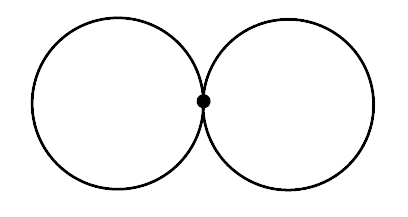
\includegraphics[scale=0.5]{vac_fluc}
\end{center}

\noindent Now, first order corrections to $\frac{\delta^2 Z[J]}{\delta J(x_1)\delta J(x_2)}$ can be obtained by expanding $Z_0[J]$ upto 3rd order.

$$\int d^Dy\,\frac{\delta^2}{\delta J^4(x_1)\delta J^4(x_2)}\frac{\delta^4}{\delta J^4(y)}\frac{1}{3!}\left(\frac{1}{2}\int d^Dz_1\int d^Dz_2J(z_1)G_0(z_1-z_2)J(z_2)\right)^3$$

\noindent which gives us six factors of source $J$ at $z_1\cdots z_6$, and six derivatives, one at $x_1$, one at $x_2$ and four at $y$. The non-vanishing Feynman diagrams are, 

\begin{center}
    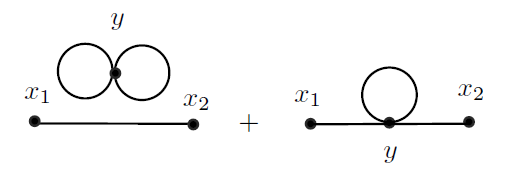
\includegraphics{green_1st}
\end{center}

\noindent The first term is $G_0(x_1-x_2)\left[\frac{-\lambda}{8}\int d^Dy\,(G_0(y-y))^2\right]$ and the second term is $\left(\frac{-\lambda}{8}\right)S\int d^Dy\,G_0(x_1-y)G_0(y-x_2)$. Here, $S=4\times 3\times 1=12$ (4 ways of contracting one external point to one of the lines attached to the vertex, 3 ways to do it for another point, 1 way to contract the two leftover lines to the vertex). Therefore, the full propagator becomes

\begin{center}
    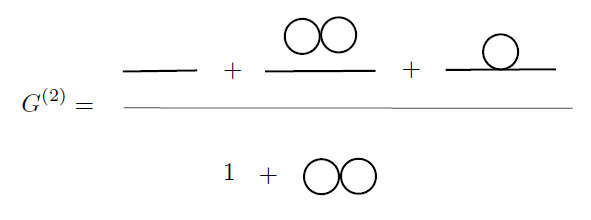
\includegraphics[scale=0.75]{cancel_1}
    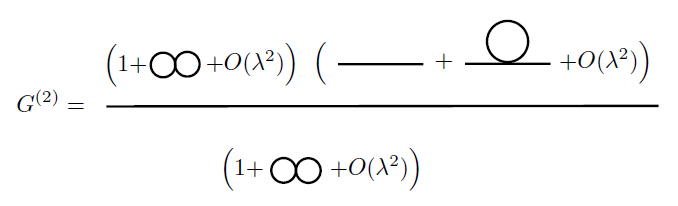
\includegraphics[scale=0.75]{cancel_2}
\end{center}

\noindent The vaccuum fluctuation cancels out. 

$$G^{(2)}(x_1-x_2)=G_0^{(2)}(x_1-x_2)-\frac{\lambda}{2}\int d^Dy\,G_0^{(2)}(x_1-y)G_0^{(2)}(y-x_2)+\mathcal{O}(\lambda^2)$$

\noindent Diagramatically, each vertex contributes $\lambda$ to the amplitude, and propagation between two internal points $z_1$ to $z_2$ is given by the correlation function. The result is then integrated over each internal point and internal loop.

\part{Application in Condensed Matter : Ising model}

\chapter{Phase Transitions}
The Ising model provides a simple description of a magnet, stating that in a lattice in $d$ spatial dimension containing $N$ sites, each site is occupied by a state with a magnetic moment (spin). The spins, $s_i$, take the value +1 or -1. This collection of spins has Hamiltonian $\mathcal{H}=-B\sum_i s_i- J\sum_{<ij>}s_is_j$. The first term arises due to the effect of an external magnetic field on the spins, while the second is an interaction term between nearest neighbours. $J>0$ implies that the adjacent spins prefer to be aligned, and the system is a ferromagnet.\\

\noindent In the canonical ensemble, the probability of sitting in a configuration of spins $\{s_i\}$ is given by $p[s_i]=\frac{e^{-\beta E[s_i]}}{Z}$, where $\beta=\frac{1}{T}$ and the normalization factor $Z=\sum_{s_i}e^{-\beta E[s_i]}$ is the partition function.\\ 

\noindent A quantity of interest is the average magnetization $m$, which will play the role of the scalar field later on. It takes values between -1 (low temperature, ordered spins) and +1 (high temperature, random spins). The thermodynamic free energy is defined as $F=-T\log Z$, therefore, if we first sum over all configurations with fixed average magnetisation and subsequently sum over all possible m, we can redefine $Z=\sum_me^{-\beta F(m)}$.

\section{Mean Field Theory}
Since the average magnetization for N lattice sites is $m$, we can construct an average energy of $\frac{E}{N}=-Bm-\frac{1}{2}Jqm^2$, where $q=2d$ is the number of nearest neighbours in $d$ dimensions. A configuration with $N_\uparrow$ up spins and $N_\downarrow=N-N_\uparrow$ down spins has magnetization $m=\frac{2N_\uparrow-N}{N}$ and the number of such configurations is given by $\Omega=\frac{N!}{(N_\uparrow!)(N-N_\uparrow)!}$. Using Stirling's approximation, the average free energy is obtained as

$$f(m)\approx -Bm-\frac{1}{2}Jqm^2+T\left(\frac{1}{2}(1+m)\log(1+m)+\frac{1}{2}(1-m)\log(1-m)\right)$$

\noindent When $m$ is small, we can Taylor expand upto

$$f(m)\approx -Bm+\frac{1}{2}(T-Jq)m^2+\frac{1}{12}Tm^4$$

\noindent The critical temperature is $T_c=Jq$. For $B=0$, temperatures above $T_c$ gives a minimum at $m=0$. However, as the temperature is reduced below $T_c$, the minima now lie at $m=\pm m_0$.

\begin{center}
    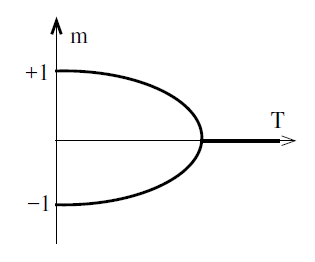
\includegraphics[scale=0.75]{mvsT_B0}
\end{center}

\noindent The magnetization turns off abruptly at the critical temperature, and remains zero for all higher temperatures. This kind of sharp change is characteristic of a second order phase transition.\\

\noindent If $B\neq 0$, we again Taylor expand the free energy and differentiate it. Now, the ground state of the system, i.e. the global minimum of $f(m)$, does not qualitatively change as we vary the temperature. At high temperatures, the magnetisation asymptotes smoothly to zero. Whether the system chooses $m=+1$ or $m=-1$ depends solely on the sign of the magnetic field. There is no phase transition as a function of temperature.

\begin{center}
    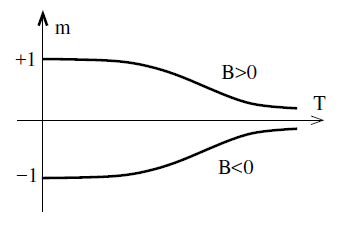
\includegraphics[scale=0.75]{mvsT_B!0}
\end{center}

\noindent Keeping $T$ fixed at a temperature lower than $T_c$, if $B$ is varied continuously such that it changes its sign, the magnetization jumps discontinuously. This is a first order phase transition. For $T>T_c$, any change in $B$ is possible without suffering a phase transition.

\section{Critical Exponents}
The mean field theory is strongly dependent on the dimensionality of the system. For $d=1$, MFT fails completely. Thus the lower critical dimension is 1. There are no phase transitions. For $d=2$ and $d=3$ phase transitions occur, but quantitative predictions around the critical temperature are wrong. For $d>4$, MFT provides correct answers. Thus, the upper critical dimension is 4.\\

$$c=\left[\beta^2\frac{\partial^2}{\partial\beta^2}\log Z\right]_{T\rightarrow T_c}\implies c\sim|T-T_c|^{-\alpha}\hspace{1cm}\alpha=0$$
$$\left[\frac{\partial f}{\partial m}\right]_{B=0}=0\implies m\sim(T-T_c)^\beta\hspace{1cm}\beta=\frac{1}{2}$$
$$\chi=\left[\frac{\partial m}{\partial B}\right]_{T\rightarrow T_c}\implies\chi\sim\frac{1}{|T-T_c|^\gamma}\hspace{1cm}\gamma=1$$
$$\left[\frac{\partial f}{\partial m}\right]_{T=T_c}=0\implies m\sim B^\frac{1}{\delta}\hspace{1cm}\delta=3$$\\

\noindent The coefficients $\alpha$, $\beta$, $\gamma$ and $\delta$ are known as critical exponents. In $d=3$, the Ising model cannot be solved analytically. The numerical values obtained are $\alpha=0.1101$, $\beta=0.2364$, $\gamma=1.2371$ and $\delta=4.7898$.

\noindent The phase transitions for liquid-gas transformations is similar to the Ising model. Here, the critical point is at $T_c=373\,^\circ C$ and $p_c=218$ atm. Similarly, the criritical exponents can be computed using MFT. Calculating $v_\text{gas}-v_\text{liquid}$ gives us $\beta=\frac{1}{2}$ for constant pressure and $\delta=3$ for constant temperature. Analogous to magnetic susceptibilty is the compressibilty $\kappa$, which gives $\gamma=1$. Again, these values are incorrect for $d=2$ and $d=3$.\\

\noindent This is not a coincidence. For a second order phase transition, the underlying microscopic structure is not important. The fact that many different systems can be decribed by the same physics of critical exponents is called universality. This is largely dictated by the symmetries of the system. 

\section{Landau-Ginzburg Theory}
The previous approach treated magnetization to be a constant. In the Landau-Ginzburg theory, it is promoted to the status of a field as its spatial variations are taken into account. The lattice is coarse-grained into boxes of side $a$ and $N'$ sites, each with magnetization $m(\boldsymbol{x})$. As per the definition of a field, $m(\boldsymbol{x})$ is treated to be continuous. Thus, the partition function now becomes an integral over all field configurations, $Z=\int \mathcal{D}m(\boldsymbol{x})\,e^{-\beta F[m(\boldsymbol{x})]}$. The free energy becomes a functional, and mimics the behaviour of the previously studied $\phi^4$ theory, just with spacetime derivatives replaced by normal Euclidean gradient operators. If we replace $m$ by $\phi$,

$$F[\phi(\boldsymbol{x})]=\int d^dx\, \left[\frac{1}{2}\alpha_2 \phi^2+\frac{1}{4}\alpha_4 \phi^4+\frac{1}{2}\gamma(\nabla\phi)^2\right]$$

\noindent $\alpha_2$, $\alpha_4$ and $\gamma$ are functions of temperature.\\

\noindent I will first start with the free field expansion, i.e. $\alpha_4=0$. $\alpha_2$ is redefined as $\mu^2=T-T_c$. The quartic term becomes important as $T\rightarrow T_c$ and its effects cannot be ignored, so the results will not hold when $\mu^2\rightarrow 0$.\\

\noindent The Fourier transform of the field $\phi(\boldsymbol{k})=\int d^dx\, e^{-i\boldsymbol{k}\cdot\boldsymbol{x}}\phi(\boldsymbol{x})$. Since the field is real, $\phi^*(\boldsymbol{k})=\phi(\boldsymbol{-k})$.

\begin{align*}
    \begin{split}
        F[\phi(\boldsymbol{k})]&=\frac{1}{2}\int\frac{d^dk_1}{(2\pi)^d}\int\frac{d^dk_2}{(2\pi)^d}\int d^dx\,(-\gamma\boldsymbol{k}_1\cdot\boldsymbol{k}_2+\mu^2)\phi(\boldsymbol{k}_1)\phi(\boldsymbol{k}_2)e^{i(\boldsymbol{k}_1+\boldsymbol{k}_2)\cdot\boldsymbol{x}}\\
        &=\frac{1}{2}\int\frac{d^dk}{(2\pi)^d}\,(-\gamma k^2+\mu^2)\phi(\boldsymbol{k})\phi^*(\boldsymbol{k})
    \end{split}
\end{align*}

\noindent The free energy decomposes into individual modes. The path integral then becomes

$$Z=\prod_k\int d\phi(\boldsymbol{k})\int d\phi^*(\boldsymbol{k})\,e^{-\frac{\beta}{2}\int\frac{d^dk}{(2\pi)^d}\,(\gamma k^2+\mu^2)|\phi(\boldsymbol{k})|^2}$$

The integral is converted to sum in finite volume $V$, and the Gaussian integral is applied for each $\boldsymbol{k}$.

$$Z=\prod_k\sqrt{\frac{2\pi V}{\beta(\gamma k^2+\mu^2)}}$$\\

\noindent The spatial fluctuations around the ground state are captured by the correlation function. Borrowing results from the previous chapter,

$$\left[\frac{1}{\beta^2}\frac{\delta^2\log Z}{\delta B(\boldsymbol{x})\delta B(\boldsymbol{y})}\right]_{B=0}=\langle\phi(\boldsymbol{x})\phi(\boldsymbol{y})\rangle$$
$$Z[B]=e^{-\beta F}e^{\frac{\beta}{2}\int d^dx\int d^dy\,B(\boldsymbol{x})G(\boldsymbol{x}-\boldsymbol{y})B(\boldsymbol{y})}$$\\

\noindent The Green's function is rotationally invariant, so we can put $|\boldsymbol{x}-\boldsymbol{y}|=r$. Introducing the correlation length as $\xi^2=\frac{\gamma}{\mu^2}$, the Green's function can be solved as a function of $r$ using Bessel functions. 

$$G(r)\sim\frac{1}{r^{d-2}}\hspace{1cm}\text{when }r\ll\xi$$
$$G(r)\sim\frac{e^{-\frac{r}{\xi}}}{r^{\frac{d-1}{2}}}\hspace{1cm}\text{when }r\gg\xi$$\\

\noindent It can be inferred that all correlations die off exponentially quickly at distances $r\gg\xi$. In contrast, for $r\ll\xi$ there is a much slower, power-law fall-off. In this sense, $\xi$ provides a characteristic length scale for the fluctuations. In a given thermal ensemble, there wil be patches where the magnetisation is slightly higher, or slightly lower than the average $\langle m\rangle$. The size of these patches will be no larger than $\xi$. Close to the critical point, the system will undergo fluctuations of arbitrarily large size. This is the essence of a second order phase transition.

\chapter{Renormalization Group}
\section{UV Cutoff}
Even though the field is considered to be continuous, it ultimately arose from a lattice, so it can't vary on scales shorter than $a$. This means that the Fourier modes must vanish for suitably high momentum, i.e. $\phi(\boldsymbol{k})=0$ for $|\boldsymbol{k}|>\Lambda=\frac{\pi}{a}$. $\Lambda$ is called the ultraviolet cutoff.\\

\noindent Suppose that we only care about physics on long distance scales, $L$. Then we have no interest in the Fourier modes $\phi(\boldsymbol{k})$ with $k\gg\frac{1}{L}$. This suggests that we can write down a different theory, one that has a lower cut-off, $\Lambda'=\frac{\Lambda}{\zeta}$.\\

\noindent The Fourier modes can be written as $\phi(\boldsymbol{k})=\phi_-(\boldsymbol{k})+\phi_+(\boldsymbol{k})$, where $\phi_-(\boldsymbol{k})$ describe the long wavelength fluctuations and $\phi_+(\boldsymbol{k})$ describe the short wavelength fluctuations that we don't care about. $\phi_-(\boldsymbol{k})$ is non-vanishing for $k<\Lambda'$, whereas $\phi_+(\boldsymbol{k})$ is non-vanishing for $\Lambda'<k<\Lambda$. Then, the free energy is written in Fourier space which can be decomposed as,

$$F[\phi(\boldsymbol{k})]=F_0[\phi_-(\boldsymbol{k})]+F[\phi_+(\boldsymbol{k})]+F_I[\phi_-(\boldsymbol{k}),\phi_+(\boldsymbol{k})]$$. 

\noindent The third term mixes the short and long wavelength modes. The partition function becomes,

\begin{align*}
    \begin{split}
        Z&=\int\prod_{k<\Lambda'}d\phi_-(\boldsymbol{k})\,e^{-F_0[\phi_-(\boldsymbol{k})]}\int\prod_{\Lambda'<k<\Lambda}d\phi_+(\boldsymbol{k})\,e^{-F_0[\phi_+(\boldsymbol{k})]}e^{-F_I[\phi_-(\boldsymbol{k}),\phi_+(\boldsymbol{k})]}\\
        &=\int\mathcal{D}\phi_-\,e^{-F'[\phi_-]}
    \end{split}
\end{align*}

\noindent We cannot yet compare the original theory with the scaled theory. This is because the theory is defined by both the free energy and the UV cut-off, and the two theories have different cut-offs. This means that the original theory can describe things that the new theory cannot, namely momentum modes above the UV cut-off.\\

\noindent To remedy this, the momenta in the new theory is scaled as $\boldsymbol{k}'=\frac{\boldsymbol{k}}{\zeta}$. Now $\boldsymbol{k}'$ takes values up to $\Lambda$, as $\boldsymbol{k}$ did in the original theory. The counterpart of this scaling in real space is $\boldsymbol{x}'=\frac{\boldsymbol{x}}{\zeta}$. This implies we are observing the system in larger length scales. Finally, the fields are also scaled as $\phi'(\boldsymbol{x}')=\sqrt{\gamma'}\phi(\boldsymbol{x})$ to normalize the coefficient of the gradient term. The full scaled free energy takes the form,

$$F_\zeta[\phi']=\int d^dx\, \left[\frac{1}{2}(\nabla\phi')^2+\frac{1}{2}\mu^2(\zeta)\phi'\,^2+g(\zeta)\phi'\,^4\right]$$

\noindent The coupling constants `flow' as $\zeta$ increases. The original constants are evaluated at $\zeta=1$.

\section{Fixed Points}
If we keep on integrating out short distance degrees of freedom to generate a new theory again and again, there are essentially two possibilities - we could flow off to infinity, or we could converge towards a fixed point. These are points which are invariant under a RG transformation. Fixed points describe theories that have no characteristic scale. If the original theory had a correlation length scale $\xi$, then the renormalised theory has a length scale $\xi'=\frac{\xi}{\zeta}$. Fixed points must therefore have either $\xi=0$ or $\xi=\infty$.\\

\noindent In the disordered phase, with $T>T_c$, enacting an RG flow reduces the correlation length, which is equivalent to increasing the temperature. As shown in the picture below, the spins become more randomized.

\begin{center}
    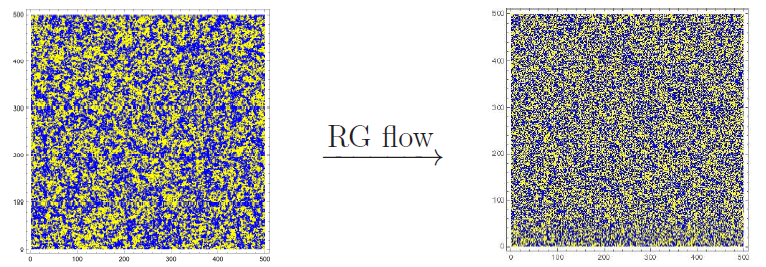
\includegraphics[scale=0.75]{disordered_rg}
\end{center}

\noindent Similarly, in the ordered phase also the RG flow reduces the correlation length. The end point at $\xi=0$ corresponds to the zero temperature limit. The spins become more aligned.

\begin{center}
    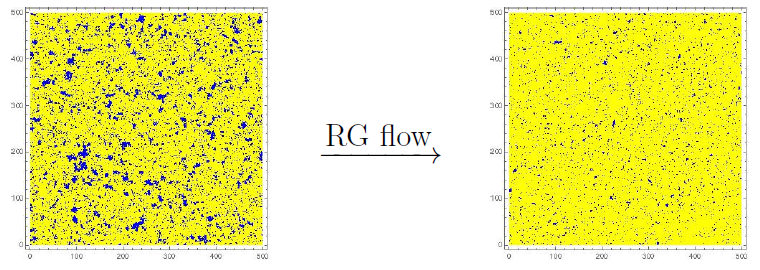
\includegraphics[scale=0.75]{ordered_rg}
\end{center}

\noindent Theories with $\xi=1$, occur at a critical point where the theory contains fluctuations on all length scales. Now, if we do an RG flow, the theory remains invariant. The configuration itself doesn't stay the same as it merely a representative configuration in the ensemble. However, as the fluctuations on small distance scales shrink away due to RG, they are replaced by fluctuations coming in from larger distance scales. In terms of visual configurations,

\begin{center}
    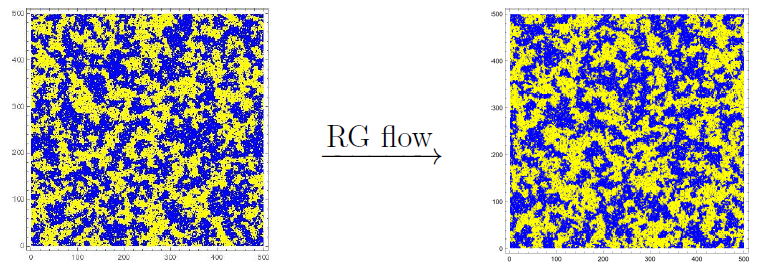
\includegraphics[scale=0.75]{critical_rg}
\end{center}

\noindent There are an infinite number of ways we can move away from the fixed point. If we move in some of these directions, the RG flow will take us back towards the fixed point. These deformations are called irrelevant because if we add any such terms to the free energy we will end up describing the same long-distance physics. In contrast, there will be some directions in which the RG flow will sweep us away from the fixed point. These deformations are called relevant because the long-distance physics will be different. Finally it's possible we simply end up on another fixed point. Such deformations are called marginal.

\section{Beta Functions}
Beta functions describe the flow of the coefficients of the field equation. After parameterizing the UV cutoff as $\Lambda'=\Lambda e^{-s}$, the beta functions are calculated by taking the derivative w.r.t. $s$.\\

\noindent For a free theory, there is no mixing between different coefficients. Any one does not induce a flow in the other. However, this no longer holds if the theory is interacting. Using Feynman rules, I have evaluated coefficients upto second order.

$$\mu^2(\zeta)=\zeta^2\left(\mu_0^2+12g_0\int_\frac{\Lambda}{\zeta}^\Lambda \frac{d^dq}{(2\pi)^d}\frac{1}{q^2+\mu_0^2}\right)$$
$$g(\zeta)=\zeta^{4-d}\left(g_0-36g_0^2\int_\frac{\Lambda}{\zeta}^\Lambda \frac{d^dq}{(2\pi)^d}\frac{1}{(q^2+\mu_0^2)^2}\right)$$\\

\noindent For small $s$, we have $\frac{d}{ds}\int_{\Lambda e^{-s}}^\Lambda dq\,f(q)\approx \Lambda f(\Lambda)$. Therefore, the beta functions become

$$\frac{d\mu^2}{ds}=2\mu^2+\frac{3g}{2\pi^2}\frac{\Lambda^4}{\Lambda^2+\mu^2}$$
$$\frac{dg}{ds}=-\frac{9g^2}{2\pi^2}\frac{\Lambda^4}{(\Lambda^2+\mu^2)^2}$$\\

\noindent The beta function for $\mu^2$ has two terms. The first term comes from the scaling procedures in RG, while the second comes from integrating out high momentum modes. Meanwhile, the beta function for $g$ only has a single term. There is no linear term in it because it was marginal under scaling, but it does receive a contribution when we integrate out the high momentum modes at second order.

\part{A Few Other Statistical Field Theories}

\chapter{Fermi Gas}
For the system of $N$ free fermions, we write the Hamiltonian $\hat{H}=\sum_\alpha E_\alpha\hat{a}^\dagger_\alpha\hat{a}_\alpha$ on $|\alpha\rangle$, a basis of a complete set of one-particle states, where the index labels the states by increasing order of energies, $E_1<E_2<\cdots$. Since we are dealing with fermions, we cannot put more than one particle in each state. Thus the state the lowest energy is obtained by filling up all the first $N$ single particle states. Let $|\text{gnd}\rangle$ denote this ground state.

$$|\text{gnd}\rangle\equiv|\overbrace{11\cdots 1}^N 00\cdots\rangle=\left(\prod_{\alpha=1}^N\hat{a}^\dagger_\alpha\right)|0\rangle$$

\noindent The energy of this state is $E_\text{gnd}=E_1+\cdots+E_N$. The energy of the top-most occupied single particle state $E_N$, is called the Fermi energy of the system and the set of occupied states is called the Fermi sea.\\

\noindent An excited state is obtained by removing one particle from the single particle state $N$ (thus leaving a hole behind) and putting the particle in the unoccupied single particle state $N+1$. This is a state with one particle-hole pair.

$$|\psi\rangle\equiv|\overbrace{11\cdots 1}^{N-1}0100\cdots\rangle=\hat{a}^\dagger_{N+1}\hat{a}_N|\text{gnd}\rangle$$

\noindent The energy of this state is $E_\psi=E_1+\cdots+E_{N-1}+E_{N+1}$. The excitation energy is $\varepsilon_\psi=E_\psi-E_\text{gnd}>0$.\\

\begin{center}
    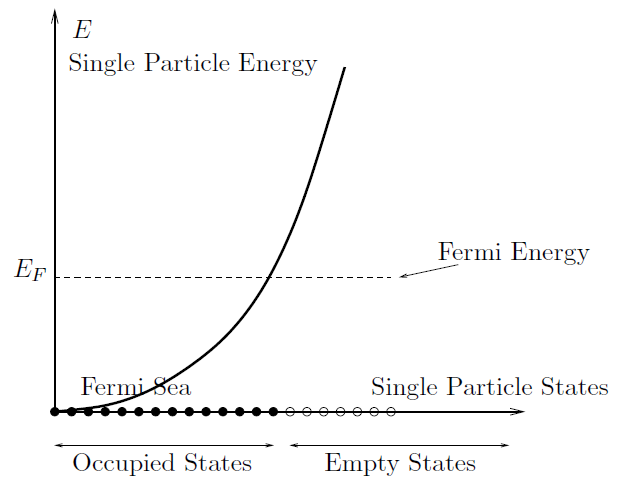
\includegraphics[scale=0.8]{fermi}
\end{center}

\noindent It is more reasonable to use $|\text{gnd}\rangle$ instead of $|0\rangle$ as the reference state. An operator $\hat{b}_\alpha=\hat{a}^\dagger_{\alpha}$ is introduced. Since these are fermionic operators, anticommutation relations $\{\hat{a}_{\alpha},\hat{a}^\dagger_{\alpha'}\}=\delta_{\alpha\alpha'}$ and $\{\hat{b}_{\beta},\hat{b}^\dagger_{\beta'}\}=\delta_{\beta\beta'}$ hold for $\alpha,\alpha'>N$ and $\beta,\beta'\leq N$.\\

\noindent Relative to the $|\text{gnd}\rangle$, $\hat{a}^\dagger_\alpha$ and $\hat{b}^\dagger_\beta$ behave like creation operators for electrons and holes respectively. An arbitrary excited state has the form

$$\hat{a}^\dagger_1\cdots\hat{a}^\dagger_m\hat{b}^\dagger_1\cdots\hat{b}^\dagger_n=|\alpha_1\cdots\alpha_m\beta_1\cdots\beta_n;\text{gnd}\rangle$$

\noindent This state has $m$ electrons and $n$ holes. $m$ is always equal to $n$. On the other hand, the ground state is annihilated by $\hat{a}_\alpha$ and $\hat{b}_\beta$.

$$\hat{a}_\alpha|\text{gnd}\rangle=\hat{b}_\beta|\text{gnd}\rangle=0$$\\

\noindent The Hamiltonian is normal ordered relative to the empty state, i.e. $\hat{H}|0\rangle=0$, but is not normal ordered relative to the ground state. The particle-hole transformation enables us to write,

$$\hat{H}=E_\text{gnd}+\sum_{\alpha>N}E_\alpha\hat{a}^\dagger_\alpha\hat{a}_\alpha-\sum_{\beta\leq N}E_\beta\hat{b}^\dagger_\beta\hat{b}_\beta$$

\noindent The number operator is given by

$$\hat{N}=N+\sum_{\alpha>N}\hat{a}^\dagger_\alpha\hat{a}_\alpha-\sum_{\beta\leq N}\hat{b}^\dagger_\beta\hat{b}_\beta$$

\noindent Electrons raise the energy while holes reduce it. Imposing the condition that the Hamiltonian conserves the particle number, i.e. $[\hat{N},\hat{H}]=0$, we see that for every particle that is removed a hole must be created. Hence particles and holes can only be created in pairs.

\chapter{Goldstone Bosons}
The phases of matter are characterised by two symmetry groups - $G$, the symmetry of the free energy of the system and $H$, the symmetry of the ground state.\\

\noindent This structure can be seen in the Ising model. When $B=0$, the free energy has a $G=\mathbb{Z}_2$ symmetry. In the disordered phase this symmetry is unbroken, i.e. $H=\mathbb{Z}_2$ also. In contrast, in the ordered phase the symmetry is spontaneously broken as the system must choose one of two ground states. Here $H$ has no symmetry group.\\ 

\noindent Whenever a discrete symmetry group is spontaneously broken, it results in multiple ground states. One can move from one ground state to another by acting with the broken generators of $G$. The different phases of matter within this class are characterised by $H$, therefore there must be a phase transition, whenever $H$ changes.\\

\noindent The theory of $N$ real scalar fields with $O(N)$ symmetry can be used to demonstrate spontaneuos symmetry breaking in condensed matter systems. The $N=2$ models come under the $XY$-universality class. Bose-Einstein condensates and superfluids are described in this way.\\ 

\noindent It is convenient to pair the two real fields as one complex field as $\psi=\phi_1+i\phi_2$. This is now invariant under $U(1)$ transformations, $\psi'=e^{i\theta}\psi$. Unlike the Ising model, where there were only two possible ground states, in a continuous symmetry there are an infinite number of ground states.\\ 

\noindent The minimum of the free energy constrains only the magnitude of $\psi$ which is given by $\langle|\psi|\rangle=M_0=\sqrt{\frac{-\mu^2}{4g}}$. However, minimising the free energy does not determine the direction of $\psi$. We are left with a space of ground states which is the sphere $\mathbb{S}^{N-1}=\frac{O(N)}{O(N-1)}$. In a general sense, the manifold of ground states is given by $\frac{G}{H}$. Each point on the sphere, parameterizes the direction of $\psi$ and has the same energy.\\

\noindent We can consider configurations in which we stay within the space of ground states, but the direction varies in space. For such configurations, the part of the free energy $f(\psi)=\mu^2|\psi|^2+g|\psi|^4$ remains minimised, but we pick up contributions from the gradient terms $\nabla\psi^*\nabla\psi$.\\

\noindent These kind of excitations, which arise from the spontaneous breaking of continuous symmetries, are known as Goldstone bosons. The number of Goldstone bosons is given as $\text{dim}(G)-\text{dim}(H)$. For the $O(N)$ models, the number is $\frac{1}{2}N(N-1)-\frac{1}{2}(N-1)(N-2)=N-1$, which is the dimensionality of $\mathbb{S}^{N-1}$.\\

\begin{center}
    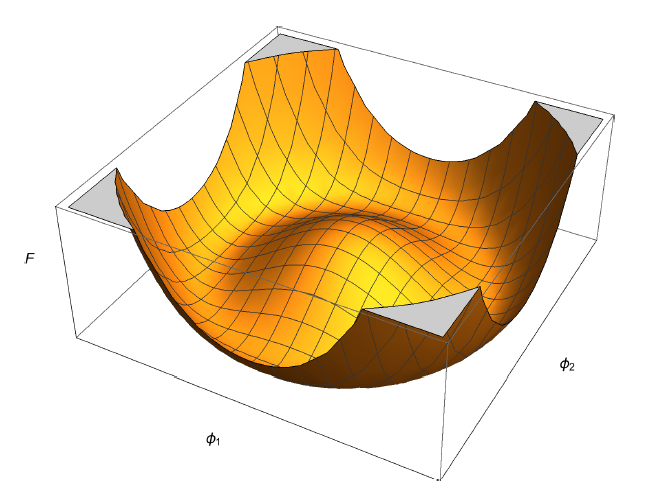
\includegraphics[scale=0.8]{ssb}
\end{center}

\noindent For the $XY$ class, in the ordered phase we get a free energy of the form as shown above. There is a circle of minima, $\mathbb{S}^1$. If we write $\psi(\boldsymbol{x})=M(\boldsymbol{x})e^{i\theta(\boldsymbol{x})}$ and $M(\boldsymbol{x})=M_0+\bar{M}(\boldsymbol{x})$, the free energy takes the form,

$$F[M,\theta]=\int d^dx\,\frac{\gamma}{2}(\nabla\bar{M})^2+\mu^2\bar{M}^2+g\bar{M}^4+\frac{\gamma}{2}M_0^2(\nabla\theta)^2+\gamma M_0\bar{M}(\nabla\theta)^2$$

\noindent $\theta$ is the Goldstone boson.

\begin{appendices}

\chapter{Lie Groups and Algebras}
Many field theories have equations that have symmetries mimicking the symmetries of Lie groups. Elements of a Lie group are continuous in nature having an associated Lie algebra on a vector space with basis $u_i$. The Lie algebra satisfies the following properties -

$$[u_i,u_i]=0$$
$$[u_i,u_j]=-[u_j,u_i]$$
$$[u_i,[u_j,u_k]]+[u_j,[u_k,u_i]]+[u_k,[u_j,u_i]]=0 \text{ (Jacobi's identity)}$$
$$[u_i,u_j]=\sum_k c^k_{ij}u_k$$

\noindent where $c^k_{ij}$'s are the structure constants for a particular algebra. And the elements of the group are given as $Q(\theta_i)=e^{\frac{i}{2}\sum_i \theta_i u_i}$\\

\noindent For example, the group $SU(2)$ has its generators given by the Pauli matrices. $[\sigma_1,\sigma_2]=2i\sigma_3\implies c^k_{ij}=\epsilon_{ijk}$. For getting a particular representation, we can choose $\theta_i=(\theta,0,0)$.

$$e^{\frac{i}{2} \theta\sigma_1}=\begin{bmatrix} \cos\left(\frac{\theta}{2}\right) && i\sin\left(\frac{\theta}{2}\right) \\ i\sin\left(\frac{\theta}{2}\right) && \cos\left(\frac{\theta}{2}\right)\end{bmatrix}$$

\noindent We can see that this matrix satifies the requirements for a being an $SU(2)$ representation as its determinant is 1 and it is unitary.

\chapter{Ladder Operators}
Any quantized field must obey Heisenberg's uncertainty principle $[\Pi_r(\boldsymbol{x},t),\eta_s(\boldsymbol{x'},t)]=-i\delta_{rs}\delta^3(\boldsymbol{x}-\boldsymbol{x'})$, where $\eta$'s are fields and $\Pi$'s are conjugate momenta.\\

\noindent The creation and annihilation operators, collectively known as ladder operators, are respectively defined as follows.

$$\hat{a}(\boldsymbol{k})=\omega(\boldsymbol{k})\eta(\boldsymbol{k})+i\Pi(\boldsymbol{k})$$
$$\hat{a}^\dagger(\boldsymbol{k})=\omega(\boldsymbol{k})\eta(\boldsymbol{k})-i\Pi(\boldsymbol{k})$$

\noindent Where, $\omega=\sqrt{k^2+m^2}$\\

\noindent The creation operator creates a quanta of the field with momentum $\boldsymbol{k}$, while the annihilation operator destroys a quanta of the field with momentum $\boldsymbol{k}$.\\

\noindent We can define the field and conjugate momenta in terms of $\hat{a}$ and $\hat{a}^\dagger$.

$$\eta(\boldsymbol{x})=\int\frac{d^3k}{2(2\pi)^3\omega}(\hat{a}e^{-i\boldsymbol{k}\cdot\boldsymbol{x}}+\hat{a}^\dagger e^{i\boldsymbol{k}\cdot\boldsymbol{x}})$$

$$\Pi(\boldsymbol{x})=\int\frac{d^3k}{2(2\pi)^3}(\hat{a}e^{-i\boldsymbol{k}\cdot\boldsymbol{x}}-\hat{a}^\dagger e^{i\boldsymbol{k}\cdot\boldsymbol{x}})$$

\end{appendices}

\addcontentsline{toc}{chapter}{\numberline{}Bibliography}
\begin{thebibliography}{10}
    \bibitem{} Angheluta-Bauer, Luiza, \emph{Ferromagnetic Phase Transition}, Universitetet i Oslo (2018)
    \bibitem{} Belyaev, Alexander, \emph{Path Integrals in QFT}, University of Southampton (2012)
    \bibitem{} Fradkin, Eduardo, \emph{Quantum Field Theory: An Integrated Approach}, Princeton University Press (2020)
    \bibitem{} Goldstein, Herbert, et al., \emph{Classical Mechanics}, Addison-Wesley (2000)
    \bibitem{} Joshi, A.W., \emph{Elements of Group Theory for Physicists}, John Wiley and Sons (1988)
    \bibitem{} Kleinert, Hagen and Schulte-Fr\o hlinde, Verena, \emph{Critical Properties of $\phi^4$ Theories}, Freie Universit\"at Berlin (2001)
    \bibitem{} Rom$\tilde{\text{a}}$o, Jorge C., \emph{Canonical Quantization of Free Fields}, T\'ecnico Lisboa (2013)
    \bibitem{} Scherer, Michael M., \emph{Introduction to Renormalization}, University of Cologne (2018)
    \bibitem{} Tong, David, \emph{Statistical Field Theory}, University of Cambridge (2017)
    \bibitem{} Xin, Xianhao, \emph{Glashow-Weinberg-Salam Model: Electroweak Symmetry Breaking}, University of Illinois (2007)
\end{thebibliography}

\end{document}